% NOAH

Die Rahmenbedingungen für das Analoge Frontend (AFE) waren durch die Vorgängerarbeit bereits gegeben. Diese sind in \ref{sec:ausgangslage} bereits erläutert.

\subsection{Schaltungsdesign}

Das AFE ist eine Kette aus Verstärkerstufen an deren Ende ein ADC das Signal abtastet. Diese Kette ist in Abbildung \ref{fig:chain} zu sehen.

\begin{figure}[H]
    \begin{center}
        \tikzset{font={\fontsize{8pt}{12}\selectfont}}
        \begin{tikzpicture}[x=0.021\linewidth,y=0.021\linewidth]

            % AD8331

            \draw[name path=lna] (0,0) node{}
            -- (0,6) node{}
            -- (6,3) node{}
            -- cycle;

            \node at (2, 3) {13dB};
            \node at (3, -1) {LNA};

            \draw[name path=attenuator] (7, 0) node{}
            -- (7, 6) node{}
            -- (13, 6) node{}
            -- (13, 0) node{}
            -- cycle;

            \node at (10, 3) {0 to 40 dB};
            \node at (10, -1) {Attenuator};

            \draw[name path=fga] (14,0) node{}
            -- (14,6) node{}
            -- (20,3) node{}
            -- cycle;

            \node at (16, 3) {21dB};
            \node at (17, -1) {FGA};

            \draw[name path=vga] (21,0) node{}
            -- (21,6) node{}
            -- (27,3) node{}
            -- cycle;

            \node[align=left] at (23, 3) {3.5dB \\ 15.5dB};
            \node at (24, -1) {VGA};

            \draw[name path=AD8331] (-0.5, -2) node{}
            -- (-0.5, 7) node{}
            -- (27.5, 7) node{}
            -- (27.5, -2) node{}
            -- cycle;

            \node at (1.5, -3) {AD8331};

            % ISL55210

            \draw[name path=pa] (28.5,0) node{}
            -- (28.5,6) node{}
            -- (34.5,3) node{}
            -- cycle;

            \node at (30.5, 3) {28.5dB};
            \node at (31.5, -1) {PA};

            \draw[name path=ISL55210] (28, -2) node{}
            -- (28, 7) node{}
            -- (35, 7) node{}
            -- (35, -2) node{}
            -- cycle;

            \node at (30, -3) {ISL55210};

            % LTC2252

            \draw[name path=adc] (36, 0) node{}
            -- (36, 6) node{}
            -- (42, 6) node{}
            -- (42, 0) node{}
            -- cycle;

            \node[align=center] at (39, 3) {12 bit \\ 105 $\frac{MS}{s}$};
            \node at (39, -1) {ADC};

            \draw[name path=LTC2252] (35.5, -2) node{}
            -- (35.5, 7) node{}
            -- (42.5, 7) node{}
            -- (42.5, -2) node{}
            -- cycle;

            \node at (37.5, -3) {LTC2252};

            \path[name path=lineA] (0, 2) coordinate (A1) node{}
            -- (41, 2) coordinate (A2) node{};

            \path[name path=lineB] (0, 4) coordinate (B1) node{}
            -- (41, 4) coordinate (B2) node{};

            \path [name intersections={of=lineA and lna, name=CS1}];
            \path [name intersections={of=lineA and attenuator, name=CS2}];
            \draw[] (CS1-2) -- (CS2-1);
            \path [name intersections={of=lineA and fga, name=CS3}];
            \draw[] (CS2-2) -- (CS3-1);
            \path [name intersections={of=lineA and vga, name=CS4}];
            \draw[] (CS3-2) -- (CS4-1);
            \path [name intersections={of=lineA and pa, name=CS5}];
            \draw[] (CS4-2) -- (CS5-1);
            \path [name intersections={of=lineA and adc, name=CS6}];
            \draw[] (CS5-2) -- (CS6-1);

            \path [name intersections={of=lineB and lna, name=CS1}];
            \path [name intersections={of=lineB and attenuator, name=CS2}];
            \draw[] (CS1-2) -- (CS2-1);
            \path [name intersections={of=lineB and fga, name=CS3}];
            \draw[] (CS2-2) -- (CS3-1);
            \path [name intersections={of=lineB and vga, name=CS4}];
            \draw[] (CS3-2) -- (CS4-1);
            \path [name intersections={of=lineB and pa, name=CS5}];
            \draw[] (CS4-2) -- (CS5-1);
            \path [name intersections={of=lineB and adc, name=CS6}];
            \draw[] (CS5-2) -- (CS6-1);
        \end{tikzpicture}
    \end{center}
    \caption{Blockschaltbild des Analogen Frontends TODO: evtl noch DAC und pins zeichnen}
    \label{fig:chain}
\end{figure}

Diese Anordnung wurde so im Vorgängerprojekt gewählt um eine gewünschte verstellbare Verstärkung von 24 - 84 dB zu erhalten.
Da aber nicht alles so reibungslos funktionierte wie gewünscht, wurden alle Komponenten noch einmal sogrfältig durchgegangen und eine Leiterplatte gefertigt, welche die Komponenten einzeln aufbaut und die Möglichkeit hat diese so separat auszumessen.

Nur der DAC und der Spannungswandler von 5 auf 3.3 Volt war im Vorgängerprojekt so noch nicht vorhanden. Diese Komponenten wurden aufgrund der früher (Kapitel \ref{sec:ausgangslage}) genannten Mängel gewählt und implementiert.

\subsubsection{AD8331}

Der AD8331\cite{AD8331} ist ein Vorverstärker, der fixe Verstärkerstufen im Innern hat und dazu ein Dämpfungsglied, welches so eine verstellbare Verstärkung ermöglicht. Ausserdem kann wahlweise eine von zwei fixen Verstärkungen zugeschaltet werden. Dieser Aufbau ist in Grafik \ref{fig:AD8331} dargestellt.

\begin{figure}[H]
\begin{center}
    \includegraphics[trim={11.5cm 18.3cm .5cm 5cm},clip,scale=1.5]{../AD8331_8332_8334_Datasheet}
    \caption{A8331 Blockschaltbild.}
    \label{fig:AD8331}
\end{center}
\end{figure}

Der erste Verstärker erwartet ein single-ended Signal am Eingang verstärkt es um 19 dB, versieht es mit einem Bias und gibt ein differentielles Signal zurück. Nach dieser Stufe sind alle Signale differentiell.
Diese Stufe muss dann extern zum Dämpfungsglied geschaltet werden. Es wäre gut möglich hier noch extern ein Filter zuzuschalten. In dieser Anwendung wurden einfach 100n Kondensatoren dazwischen geschaltet um noch einmal DC zu blocken.
Die Dämpfung des Dämpfungsgliedes ist stufenlos von 0 bis 48 dB übder den GAIN-Pin verstellbar. Hierfür wurde ein einfacher DAC verwendet. Dazu in Abschnitt \ref{subsec:MCP4706} mehr.
Zuletzt wird ein Nachverstärker zugeschaltet der noch einmal 3.5 oder 15.5 dB verstärkt. Dies kann über den HILO-Pin gesteuert werden.
Ausserdem kann die Ausgangsspannung auf ein Maximum begrenzt werden, was nützlich ist um weitere Bauteile durch Überspannung zu schützen.

Der Ad8331 operiert bei 5V.

Die totale Verstärkung kann einfach mit den Formeln in \ref{eq:A8331_LO} und \ref{eq:A8331_HI} erhalten werden.

\begin{equation}
    G_{dB} = 50 \frac{dB}{V} \cdot V_{GAIN} - 6.5 dB, HILO = LO
\label{eq:A8331_LO}
\end{equation}

\begin{equation}
    G_{dB} = 50 \frac{dB}{V} \cdot V_{GAIN} - 6.5 dB, HILO = HI
\label{eq:A8331_HI}
\end{equation}

\subsubsection{ISL55210}
Der ISL55210\cite{ISL55210} ist ein Differentieller Verstärker. Er wird normal mit Feedbackwiderständen beschaltet, so dass man die gewünschte Verstärkung von 28.5 dB erhält.
Er hat ein GBWP von 4 Ghz was für das geplante SDR alleweil reicht, da das SDR nur bis 30 Mhz operieren soll. Bei einer Verstärkung von 28.5 dB ist das GBWP also noch lange nicht ausgereizt.
Dieser Verstärker operiert bei 3.3 Volt. Es ist also notwendig eine 5V und 3V3 Stromversorgung zu haben.

\subsubsection{LTC2252}
Es wurde der LTC2252\cite{LTC2252} mit 12 Bit als A/D-Wandler gewählt. Es ist zu evaluieren ob so eine hohe Auflösung überhaupt notwendig ist.
Mit 105 MS/s ist er sicher genug schnell um Aliasing zu verhinden, wenn man annimmt dass bei einer Cutoffrequenz von 30 MHz das Filter 9. Ordnung bei 50 Mhz um etwa 50dB gedämpft wird.
Die Beschaltung wurde aus dem Application Note übernommen. Hier wurde viel Augenmerk darauf gelegt die Anweisungen im Application Note akribisch zu befolgen. Dies war dann insbesondere im Leiterplattendesign wichtig.

\subsubsection{MCP4706}
\label{subsec:MCP4706}
Der MCP4706\cite{MCP4706} ist ein 8 bit DAC. Er wird dazu genutzt die variable Verstärkung des AD8331 einzustellen. Dieser wurde so konfiguriert dass er maximal ein Volt Ausgangsspannung hat, da dies die Grenze ist für den AD8331. Gleichzeitig verliert man zehn Skalierungsstufen, da der AD8331 als Untergrenze 40 mV erwartet. Somit geht der zulässige Wertebereich für den DAC von 11 bis 255. Dies sollte genügend dynamic Range sein. Wieviel Verstärkung das Erhöhen des Wertes am DAC um eins zum Ergebnis hat sieht man in Gleichung \ref{eq:DAC_wert}.

\begin{equation}
    \delta G_{dB} = 50 \frac{dB}{V} \cdot \frac{1}{2^8 - 1} = 0.196 dB
\label{eq:DAC_wert}
\end{equation}

Der DAC ist über $I^2 C$ bequem ansteuerbar. Dies war eine wichtige Eigenschaft die gefragt war. Zudem ist es natürlich wichtig dass der DAC rauscharm ist. Der MCP4706 hat eine simple Resistorladder, das heisst, es werden je nach Ausgangswert Widerstände dazu- oder weggeschaltet. Damit sollte die Spannung am DAC-Ausgang praktisch keine Schwankungen erfahren, oder besser gesagt: es ist nur vom Rauschen der Spannungsversorgung abhängig, wie man in \ref{eq:DAC_rauschen2} sehen kann. Nimmt man an, dass $\Delta f \xrightarrow 0$, da die Verstärkung einmal zu beginn der Übermittlung eingestellt wird und dann statisch bleibt, so sieht man dass das Rauschen vernachlässigbar wird.

\begin{equation}
    U_N = \sqrt{4 \cdot k_B \cdot T \cdot \Delta f \cdot R}, k_B = 1.38\cdot 10^{-23}\frac{J}{K}, T = 300K, R = 210k\Omega
\label{eq:DAC_rauschen}
\end{equation}

\begin{equation}
    U_N = \sqrt{4.1751\cdot 10^{-15} \cdot \Delta f}
\label{eq:DAC_rauschen2}
\end{equation}

\subsubsection{LP38798}
Der LP38798 ist ein linearer Spannungsregler mit guter Rauschdämpfung und aktivem Rippelausgleich. Er wurde anstelle eines Schaltreglers eingesetzt, da Schaltregler aufgrund ihres Funktionsprinzips tendenziell Störsignale einbringen statt, wie im Falle von Linearregler, sie zu dämpfen.
Dieser Regler im Speziellen ist auf tiefes Rauschen (5µV RMS) und einen hohen Versorgungsspannungsdurchgriff (PSRR) optimiert, weswegen er uns bei der Recherche ins Auge gestochen ist. Dies ist zur stabilen Stromversorgung der Verstärker auch bei Betrieb an einer weniger als optimalen Stromquelle von Bedeutung.
Weitere Kenndaten wie Chipgrösse, Preis und Effizienz waren bei der Auswahl von sekundärer Wichtigkeit da der Einsatz im Rahmen des Projekts auf Prototypen zur stationären Verwendung beschränkt ist.

% FRANCESCO GRAFIK PSRR UND NOISE DENSITY

Um Verbrauchsspitzen abzufangen wurde dem Regler ein Tiefpassfilter mit Kapazitäten nachgeschaltet.
Eine Umsetzung mit Schaltregler wäre prinzipiell vorstellbar. Eine solche Lösung hätte aber aufgrund der fehlenden architekturgegebenen Filterung zusätzliche externe Filter, speziell für die Schaltfrequenz aber auch als Ersatz des intrinsischen Filtereffekts, erfordert.

Beim Design der Leiterplatte wurde darauf geachtet, dass die leistungsführenden Leitungen bis an die Chipanschlüsse möglichst breit gehalten wurden. Zudem ist die Massenfläche zur besseren Abführung der abfallenden thermischen Leistung mehrfach durchkontaktiert.

\subsection{Leiterplattendesign}
\label{subsec:Leiterplattendesign}
Die Leiterplatte wurde so ausgelegt, dass alle Komponenten (VGA, LNA, ADC) des Frontends mehr oder weniger abgekapselt auf einem Board sind. Jede Komponente kann zu der weiterführenden benachbarten geschaltet werden. Wenn die Komponenten nicht gechaint werden, so können sie am Input und am Output an einen Balun angeschlossen werden. So können alle Komponenten einzeln gemessen werden. Die Baluns sind notwendig damit die differentiellen Komponenten korrekt terminiert werden und das Signal in ein single-ended Signal umgewandelt wird. Diese zweite Eigenschaft ist voraussetzung um einen VNA anschliessen zu können.

Wichtige Änderungen zum Vorgängerprojekt bestehen hier vor allem darin, dass die Groundplane optimiert wurde und die Komponenten näher zum jeweiligen Chip angeordnet wurden.

\subsubsection*{Groundplane}
Es ist wichtig dass in einer HF-Anwendung eine möglichst unbeschädigte Groundplane vorliegt. Zum einen braucht es ein fixes Referenzpotential welches sich möglichst nicht verschieben soll. Bei mehr Masse ist das einfacher, da die Ströme keine langen Wege nehmen müssen.

\subsubsection*{Leiterbahnen}
Leiterbahnen sollten so kurz wie möglich gehalten werden. Zudem sollten symmetrische Signale auch physikalisch so gehalten werden, wenn sie über längere Distanzen geführt werden. Das heisst sie sollten geometrisch nahe beieinander gehalten und symmetrisch geroutet werden. 

\subsubsection*{AD8331}
Im Datasheet zum AD8331 gibt es einige Tipps wie das Layouten gelingt. So soll Dead Copper vermieden werden und stattdessen mit Ground verbunden werden.
Die externen Komponenten an den Pins LON und LOP sowie an den Pins VOL und VOH sollten so nahe wie möglich am Chip platziert werden um Lodading-Effekte zu vermeiden.
Zudem sollten speziell die Verbindungen von LON und LOP zu VIN und VIP möglichst kurz gehalten werden um ungewünschte Effekte zu vermeiden. Dazwischen hat es einen externen Coupling-Kondensator, da danach das Signal mit einem Bias versehen wird um es in ein differentielles Signal zu erhalten.

\subsubsection*{ISL55210}
Beim ISL55210 wurden lediglich die üblichen wichtigen Design-Richtlinien befolgt. 

\subsubsection*{LTC2252}
Der ADC ist am heikelsten zu layouten. Er hat digitale sowie analoge Komponenten. Diese müssen strikt getrennt werden, um zu vermeiden, dass digitale Signale welche viel Strom brauchen die Referenzlevel für den analogen Teil verfälschen. Es sollen Querströme vermieden werden!
Hier war schon beim Vorgängerprojekt eine Diskussion, wie das Groundlayout auszusehen hat. Dazu gibt es verschiedene Artikel insbesondere einen Artikel von Analog Devices \cite{StayingWellGrounded2012} und natürlich das Datasheet des LTC2252\cite{LTC2252} welche Hinweise geben, wie das Layout zu gestalten sei. Es gibt verschiedene Ansätze wie man vorgehen sollte. Manche bevorzugen zwei komplett getrennte Groundplanes welche an einem Punkt zusammengeführt werden und manche bevorzugen es die Groundplane als ein Ganzes zu behalten. Sie sind sich alle in einem Punkt einig: Oftmals wird falsch verstanden zu welchem Ground bzw zu welcher Versorgung ein Pin der mit DGND (digital Ground) angeschrieben ist nun gehört. So gehört dieser Pin nicht an ein digitales Referenzpotential, sondern an ein analoges! Wieso dem genau so ist, ist wunderbar erklärt in \cite{StayingWellGrounded2012}, wird hier aber nicht noch einmal aufgeführt.
Es ist unter jeden Umständen zu vermeiden den DGND des ADCs an einen digitalen Ground zu hängen! Des weiteren ist die Verbindung zwischen AGND und DGND möglichst kurz zu halten um weitere parasitäre Effekte zu vermeiden.
Es wird im Datasheet explizit erwähnt dass der Ground unter und um den Chip aus einer ungestörten Plane besteht. Es sind eher 4-Layer+ empfohlen. Es wurde bei diesem Projekt versucht so gut wie möglich mit 2 Layern auszukommen.

Im LTC2252 Datasheet wird zudem erwähnt, dass digitale und analoge Signale gut getrennt werden müssen. Diese sollten sich unter keinen Umständen in die Quere kommen um parasitäre Koplungseffekte zu vermeiden. Dies macht einem der LTC2252 zum Glück sehr leicht, da die Signale im Pinout schon sinnvoll getrennt angeordnet sind.
Die Groundplane wurde hier so eingeschnitten, dass digitale Signale nicht über den analogen Bereich zurücklaufen. Dies ist in Grafik \ref{fig:groundplane_bsp} sehr schön zu sehen.

\begin{figure}[H]
\begin{center}
    \tikzset{font={\fontsize{48pt}{12}\selectfont}}
    \begin{tikzpicture}
        \node[opacity=1]{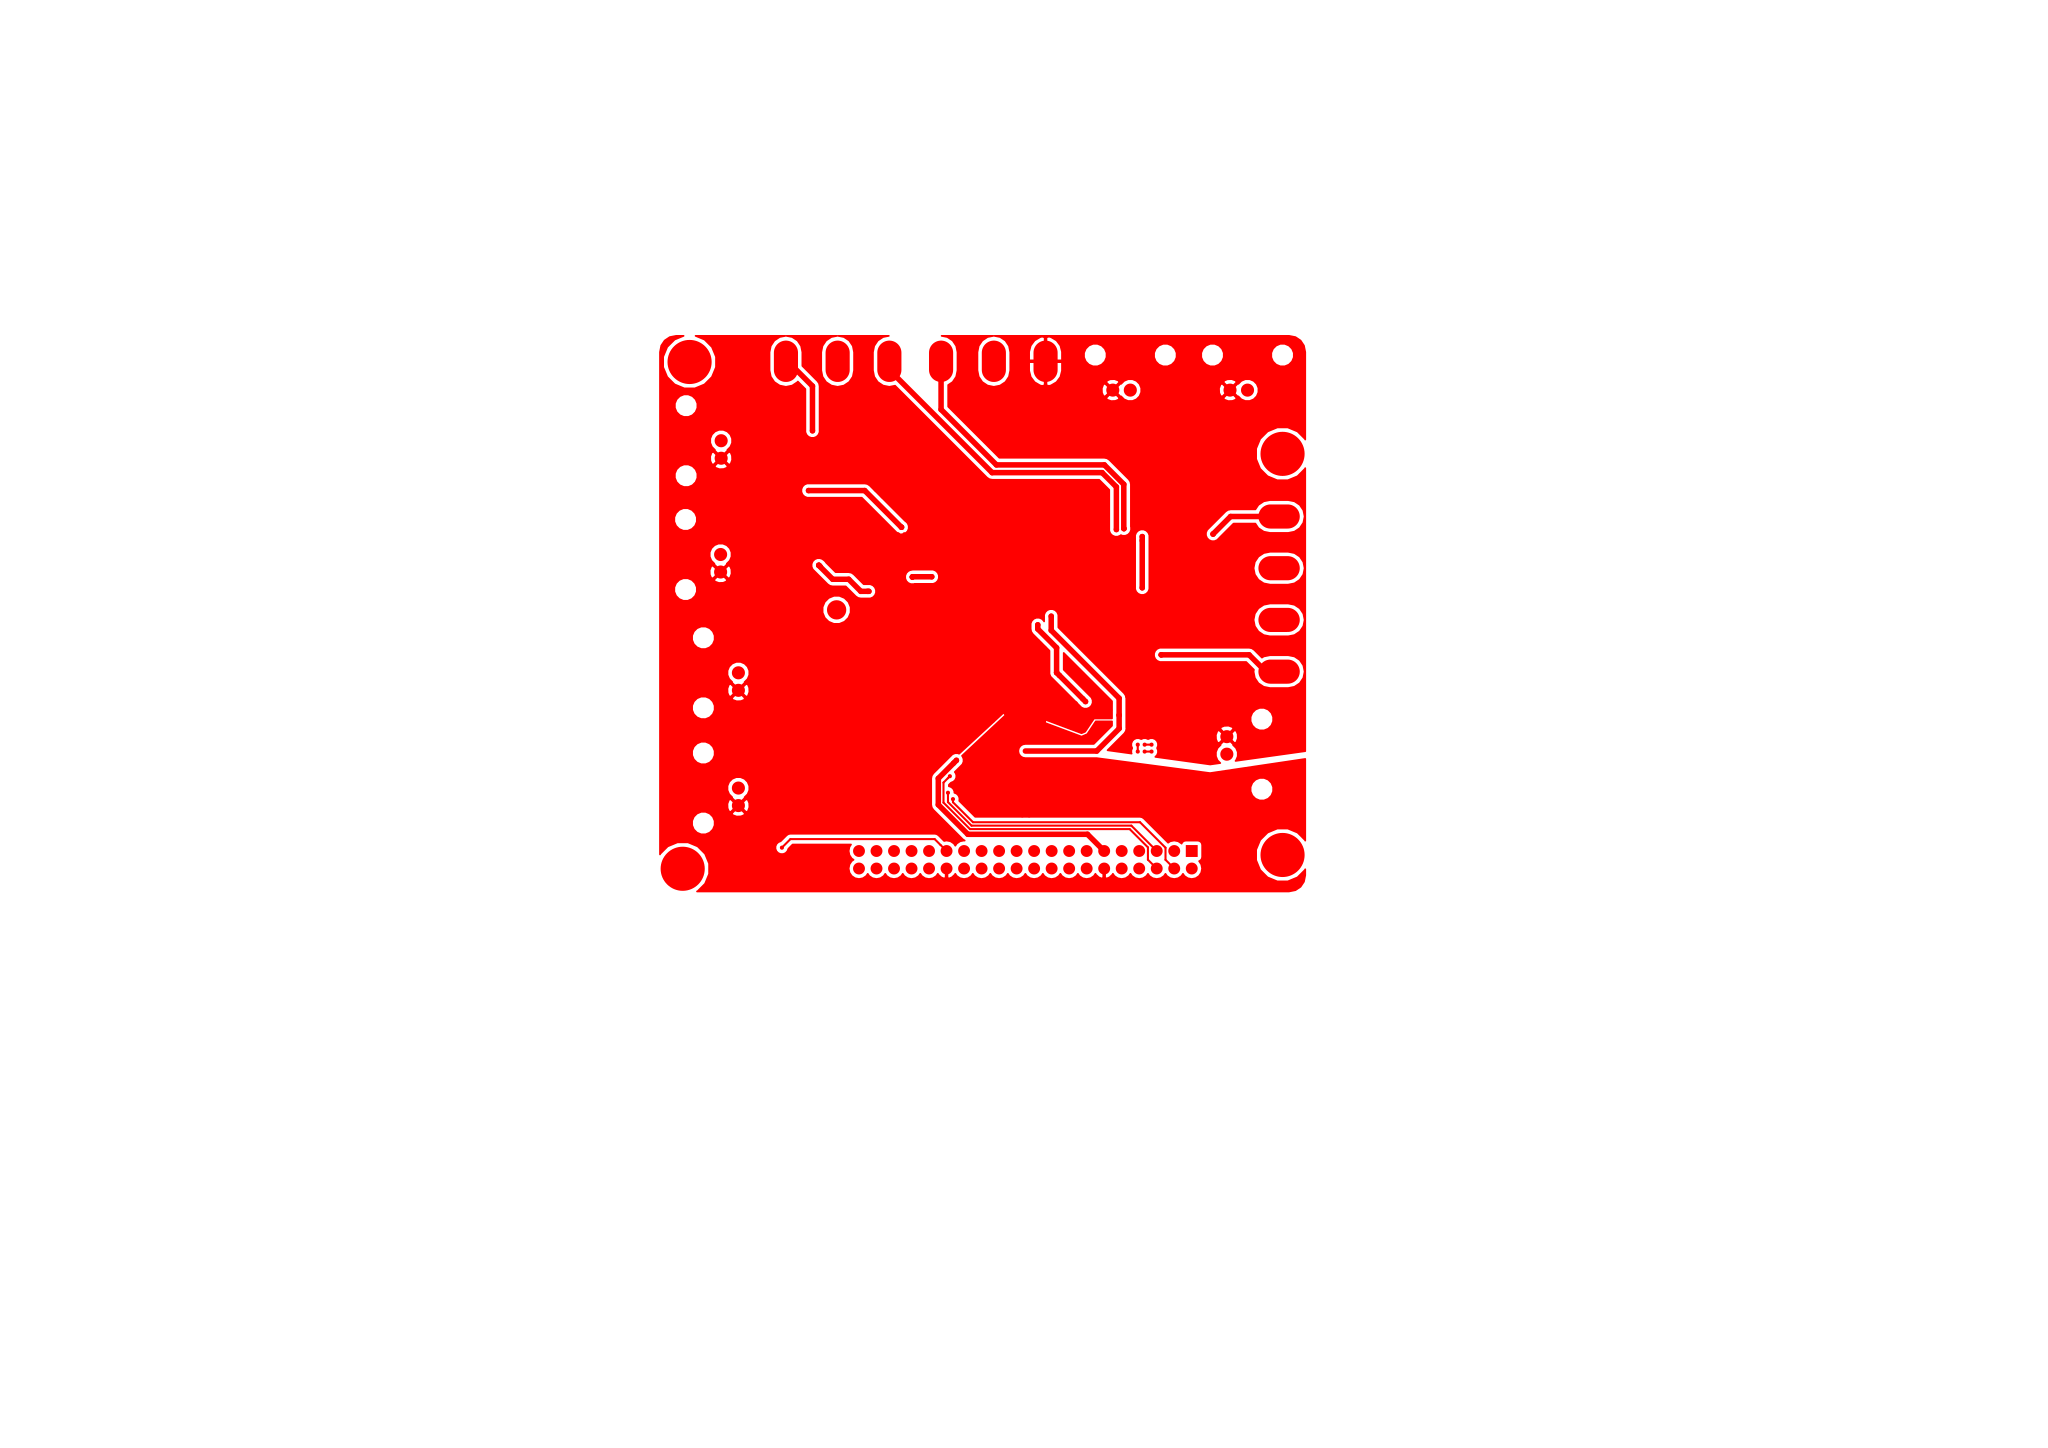
\includegraphics[trim={14cm 9.3cm 13.7cm 9.7cm},clip,scale=6]{data/images/amplifier-B_Cu}};
        \node[opacity=0.2]{\includegraphics[trim={14cm 9.3cm 13.7cm 9.7cm},clip,scale=6]{data/images/amplifier-F_Cu}};

        % Analog Area

        \draw[name path=attenuator, fill=, opacity=0.3] (-5.8, -0.5) node{}
        -- (-5.8, 5.8) node{}
        -- (5.8, 5.8) node{}
        -- (5.8, 1.8) node{}
        -- (5, 1.8) node{}
        -- (4.5, 1) node{}
        -- (4.0, 0.6) node{}
        -- (0.5, 2.3) node{}
        -- (-2.7, 2.3) node{}
        -- cycle;

        \node at (0, 4) {Analog};

        % Digital Area

        \draw[name path=attenuator, fill=, opacity=0.3] (-5.8, -1.3) node{}
        -- (-5.8, -5.8) node{}
        -- (5.8, -5.8) node{}
        -- (5.8, 1.3) node{}
        -- (5.4, 1.3) node{}
        -- (4.7, 0.2) node{}
        -- (4.2, 0) node{}
        -- (0, 1.5) node{}
        -- (-2.7, 1.5) node{}
        -- cycle;

        \node at (0, -3) {Digital};

        % ADC

        \draw[name path=attenuator] (-2, 2.2) node{}
            -- (0.5, 2.2) node{}
            -- (0.5, -0.3) node{}
            -- (-2, -0.3) node{}
            -- cycle;

        \tikzset{font={\fontsize{48pt}{12}\selectfont}}
        \node at (-0.75, 0.95) {\huge ADC};

        % DAC

        \draw[name path=attenuator] (5.8, -1.5) node{}
            -- (5, -1.5) node{}
            -- (5, -5) node{}
            -- (5.8, -5) node{};

        \node at (5, -3.25) {\huge DAC};
    \end{tikzpicture}
    \caption{Groundplane unter dem LTC2252.}
    \label{fig:groundplane_bsp}
\end{center}
\end{figure}

Speziell erwähnt im Datasheet wird vorallem der 100nF Kondensator zwischen REFH und REFL. Er darf sich nicht weiter als 1.5 mm vom Chip weg befinden. Er wird speziell aufgeführt und zum parallelen 2.2uF Kondensator wird gesagt dass dieser weiter weg sein kann, was annehmen lässt dass dies wirklich wichtig ist.